\section{Funciones del sistema}
\label{sec:CH03_FUNCIONES}

\noindent
En esta sección se identificarán todas las funcionalidades que debe tener el sistema a diseñar. Para lograr esto, se empleará una estructura de funciones, cuya finalidad es descomponer y organizar las funciones específicas que la máquina debe cumplir para realizar su propósito principal. La formulación de esta estructura, la búsqueda de principios de solución para cada función, y el análisis de las posibles combinaciones de solución, permitirán establecer un concepto óptimo de diseño la cual se presentará en la sección \ref{sec:solucion_optima} del presente trabajo de investigación.
Antes de detallar las características y funciones internas del sistema, es necesario identificar las entradas y salidas del mismo. Cualquier máquina o equipo puede describirse como una función general, representada en forma de una caja negra, donde ocurre una transformación técnica. Este proceso técnico considera tres magnitudes básicas tanto para las entradas como para las salidas: señal, energía y materia \autocite{imagen_v}.
Dentro de esta abstracción del sistema, se encontrarán las funciones que se encargarán de transformar dichas magnitudes de entrada en los resultados deseados, asegurando el cumplimiento de la función principal del sistema y los requerimientos definidos en la sec. \ref{sec:.lista de req}.

\subsection{Caja negra}

    \noindent
    Las entradas de tipo señal en la caja negra fueron elegidas de acuerdo a lo descrito en la lista de requerimientos, estas sirven para iniciar con la estimación de parámetros de motores \ac{DC}. En cambio, las salidas de tipo señal son elegidas para mostrar al usuario la información procesada, datos relevantes y gráficos relevantes luego del proceso de caracterización de un motor.
    La entrada de energía eléctrica de $220\text{VAC }60\text{Hz}$ es utilizada para energizar los actuadores, sensores y controladores involucrados en el registro de data para las pruebas con los motores \ac{DC}.
    La Figura \ref{fig:black_box} muestra la caja negra del sistema de estimación de motores \ac{DC}. Esta representación muestra las entradas y salidas de tipo energía (flecha continua), las señales (flecha punteada) y la materia (flecha de mayor grosor). A su vez, se presenta en la Tabla \ref{tab:Entradas-Salidas} el significado de cada una de las señales de entrada y de salida que se han considerado para el sistema. Considerar las señales \text{[I]} como entradas y \text{[O]} como salidas en la Tabla \ref{tab:Entradas-Salidas}.
    \begin{figure}[H]
        \centering
        \begin{tabularx}{\linewidth}{>{\centering\arraybackslash}X}
            % Fila 1: imagen
            \begin{subfigure}[t]{\linewidth}
                \centering
                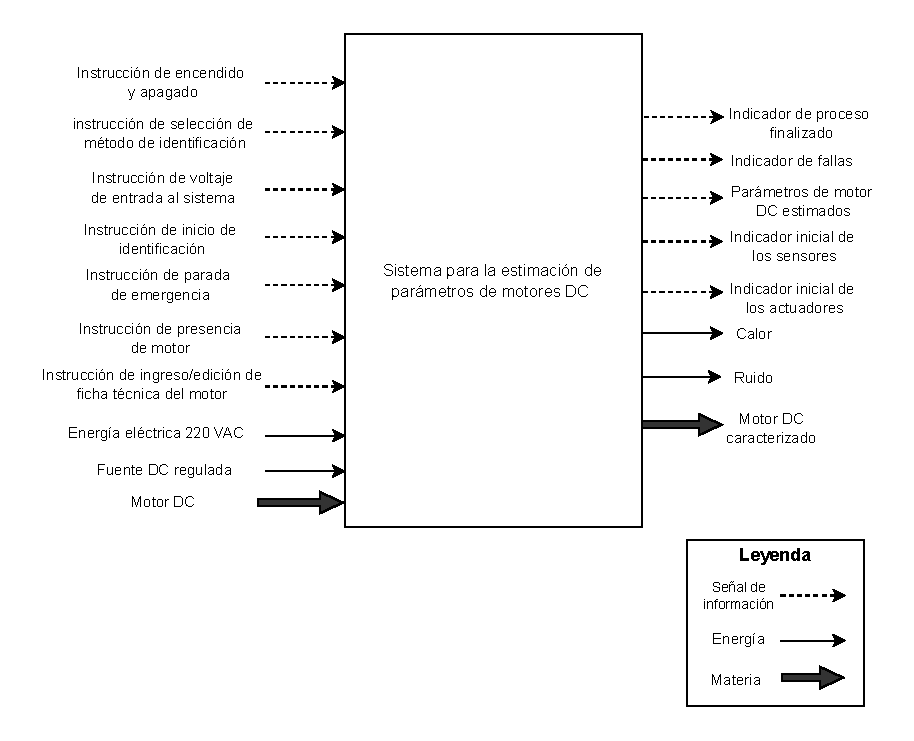
\includegraphics[width=0.8\linewidth]{CHPTRS/CH03_DICON/Fig/CH03_FIG01_EstructuraDeFunciones/01_BlackBox.pdf}
            \end{subfigure}
        \end{tabularx}
        \caption{Caja negra}
        \label{fig:black_box}
    \end{figure}
    %\begin{table}[H]
    \begin{longtblr}[theme=pucp,
        label = {tab:Entradas-Salidas},
        caption = {Descripción de señales de entrada y salida},
    ]{
        colspec = {Q[l,m]Q[l,m]Q[l,m]},
        column{1}={3cm},
        column{2}={4cm},
        column{3}={7.75cm},
        rowhead = 1, 
        rowfoot = 0,
        hlines,
        vlines
    }
    \textbf{Tipo de Señal (I/O)} & \textbf{Nombre de la señal} & \textbf{Descripción}\\
    \text{[I]}: Información & Instrucción de encendido y apagado & Señal que indicará si el sistema \ac{HW} debe ser energizado o no.\\
    \text{[I]}: Información & Instrucción de método de identificación a usar & Señal que indicará qué algoritmo de estimación se usará para hallar los parámetros.\\
    \text{[I]}: Información & Instrucción de voltaje de entrada al sistema & Señal que le indicará al controlador qué señales de entrada deberá usar para excitar al motor.\\
    \text{[I]}: Información & Instrucción de inicio de identificación & Señal que indicará el comienzo del experimento, se excita al sistema y se toman los datos de cómo varían las variables de corriente $i(t)$ y velocidad angular $\omega(t)$.\\
    \text{[I]}: Información & Instrucción de parada de emergencia & Señal que le indicará al sistema que se aisle de la fuente de energía en caso ocurra alguna falla durante el proceso de estimación.\\
    \text{[I]}: Información & Instrucción de presencia de motor & Señal que le indicará al sistema si el motor a analizar cuenta con una caja reductora o encoder, componentes que se deben tener en cuenta para acondicionar la toma de datos. Esta señal es un parámetro opcional y dependerá del tipo de motor a evaluar.\\
    \text{[I]}: Información & Instrucción de la ficha técnica del motor & Señal que indicará las características y parámetros del motor a evaluar, esto con la finalidad de que sea comparado con los valores estimados. No es necesario ingresar estos valores debido a que no todos los motores cuentan con estas especificaciones al adquirirlos.\\
    \text{[I]}: Energía & Energía eléctrica $220\text{VAC-}60\text{Hz}$ & Línea de energía eléctrica proveniente de un tomacorriente para energizar al sistema.\\
    \text{[O]}: Materia & Motor DC caracterizado & Se deberá liberar el motor del mecanismo de sujeción una vez finalizada la estimación de sus parámetros.\\
    \text{[O]}: Información & Indicador de proceso finalizado & Señal que confirma al usuario que el proceso de estimación ha concluido.\\
    \text{[O]}: Información & Indicador de fallas & Indicará si se ha detectado alguna falla durante el proceso (problemas de comunicación, datos incompletos, etc.).\\
    \text{[O]}: Información & Parámetros de motor \ac{DC} estimados & Presenta los valores calculados para los parámetros del motor.\\
    \text{[O]}: Información & Indicador inicial para los sensores & Señal que le indicará al usuario si están correctamente conectados los sensores al sistema de control.\\
    \text{[O]}: Información & Indicador inicial para los actuadores & Señal que le indicará al usuario si están correctamente conectados los actuadores al sistema de control.\\
    \text{[O]}: Energía & Calor & Energía disipada en forma de calor al energizar los motores a evaluar.\\
    \text{[O]}: Energía & Ruido & Energía en forma de ruido ocasionada por el giro de los motores una vez comenzado el proceso.\\
    \text{[O]}: Materia & Motor DC caracterizado & Se deberá liberar el motor del mecanismo de sujeción una vez finalizada la estimación de sus parámetros.
    \end{longtblr}
    %\end{table}
\subsection{Estructura de funciones}

    \noindent
    En esta sección se presentarán las interconexiones de las funciones parciales del sistema general, el cual está subdividido en dos capas principales: la capa de \ac{SW} y la capa de \ac{HW}. Dentro de la primera encontramos el dominio de la interfaz, la cual contará con las funciones necesarias para procesar los datos de entrada, enviárselos al \ac{HW} del sistema y que reciba a su vez la información necesaria para poder estimar los parametros del motor que se analice. Por otro lado, la capa \ac{HW} contará con los siguientes dominios:  (i) interfaz, (ii) comunicación, (iii) control, (iv) sensores, (v) actuadores, (vi) mecánica y (vii) energía. Cabe comentar que no se ha considerado un dominio eléctrico debido a que dicho dominio se encuentra presente en los dominios (iii), (iv), (v) e incluso en (i). Dentro de esta capa se encontrarán los componentes que interactuarán con el motor a analizar, serán los encargados de energizarlo y sensar la data que se utilizará para la estimación.
    A continuación se presentarán cada uno de los dominios con las respectivas funciones, necesarias para diseñar el estimador de parámetros de motores \ac{DC}. La estructura completa se presenta en el Anexo \ref{an:Anexo_F}.
\subsection{Dominio de Interfaz}

    \noindent
    La Figura \ref{fig:interfaz} muestra las funciones del dominio de interfaz. Las entradas de información, en su mayoría, se refieren a datos que deben ser ingresados inicialmente. Entre esas instrucciones tenemos: 
	\begin{itemize}
		\item Instrucciones de ingreso/edición de características y la ficha técnica del motor (por ejemplo, si tiene caja reductora, encoder, etc.)
		\item Instrucción para la selección de método de identificación, ya que como se planteó en el capítulo \ref{ch:CH01}, se espera implementar y comparar por lo menos 2 métodos para la estimación de parámetros de motores \ac{DC}.
		\item La señal de entrada al motor, en el capítulo \ref{ch:CH02}, se observa que para la caracterización de un motor es necesario realizar pruebas con distintos tipos de entrada para obtener con certeza cada uno de los parámetros a estimar.
		\item Una instrucción que cargará todos los datos antes mencionados para comenzar con la estimación
    \end{itemize}
    La información ingresada será procesada por los métodos del \textit{backend}, es decir la parte del sistema que se encarga de gestionar la lógica interna, de la interfaz. Dichos métodos se encargarán de gestionar y transmitir los datos a través de un protocolo de comunicación. Previo a la ejecución del algoritmo de estimación, estos métodos recibirán las entradas y, simultáneamente, registrarán los datos censados del \ac{HW} para su procesamiento. Al concluir la estimación, el sistema mostrará los resultados al usuario mediante la interfaz. Esto incluirá la visualización de gráficos con los valores estimados y los parámetros del motor. Además, se contará con un indicador de fallas dado que, si el sistema no recibe datos del controlador, no habrá información que mostrar y deberá alertar al usuario que hay alguna mala conexión. 
    \begin{figure}[H]
        \centering
        \begin{tabularx}{\linewidth}{>{\centering\arraybackslash}X}
            % Fila 1: imagen
            \begin{subfigure}[t]{\linewidth}
                \centering
                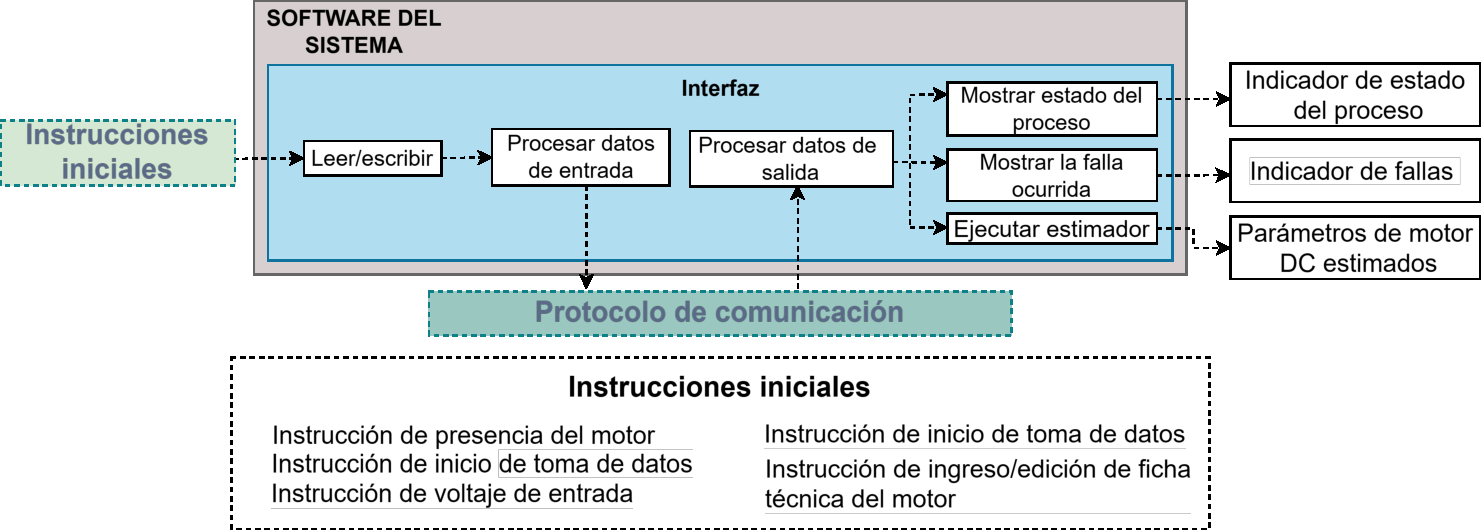
\includegraphics[width=\linewidth]{CHPTRS/CH03_DICON/Fig/CH03_FIG01_EstructuraDeFunciones/02_EstructuraDeFunciones-SW.pdf}
            \end{subfigure}
        \end{tabularx}
         \caption{Dominio de interfaz}
        \label{fig:interfaz}
    \end{figure}

\subsection{Dominio de Comunicación}

    \noindent
    Este dominio es responsable de gestionar el envío y la recepción de información entre la capa de \ac{HW} y la \ac{GUI}, a través de un protocolo de comunicación.  La información de entrada será enviada por este medio hasta llegar al controlador para comenzar con las configuraciones del \ac{HW} y posteriormente con la estimación. Los datos captados por los sensores se transmiten al dominio de la interfaz, tras ser filtrados para asegurar un procesamiento adecuado en los algoritmos de estimación. La Figura \ref{fig:comunicacion} presenta el bloque correspondiente al dominio de comunicación.
    \begin{figure}[H]
        \centering
        \begin{tabularx}{\linewidth}{>{\centering\arraybackslash}X}
            % Fila 1: imagen
            \begin{subfigure}[t]{0.65\linewidth}
                \centering
                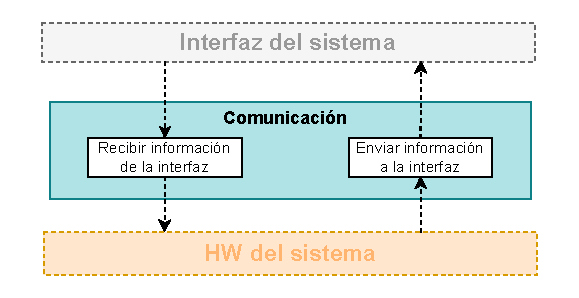
\includegraphics[width=\linewidth]{CHPTRS/CH03_DICON/Fig/CH03_FIG01_EstructuraDeFunciones/03_EstructuraDeFunciones-Com.pdf}
            \end{subfigure}
        \end{tabularx}
        \caption{Dominio de Comunicación}
        \label{fig:comunicacion}
    \end{figure}

\subsection{Dominio de Control}
\label{sec:CH04_Dominio_Cntrl}

    \noindent
    El dominio de control se encarga de gestionar las órdenes y procesar la información necesaria durante la identificación de un motor. Este dominio procesará los datos antes de enviarlos a la interfaz mediante el protocolo de comunicación seleccionado. Además, será responsable de interpretar las instrucciones iniciales proporcionadas por el usuario y de ejecutar las acciones correspondientes en los dominios de sensores y actuadores. 
    En este dominio se presentan las siguientes funcionalidades:
    \begin{itemize}
        \item Procesar la data recopilada por los sensores para la caracterización del motor y enviarla por el protocolo de comunicación elegido para la ejecución del estimador de parámetros.
        % \item Controlar el voltaje de entrada a usar para la toma de datos, para ello este dominio debe regular la fuente de voltaje que energizará al motor, esto de acuerdo al voltaje nominal del cual trabaja el motor. 
        % \item Regular y acondicionar el voltaje de entrada que será utilizado durante la toma de datos, asegurando que este se mantenga acorde al voltaje nominal del motor. Para ello, se empleará un \textit{driver} conectado al controlador, el cual, mediante un circuito externo, permitirá tanto aislar la parte de control de la de potencia como adecuar el voltaje que se inyectará al motor.
        \item Verificar que todos los sensores estén correctamente calibrados y conectados en el sistema, de modo que comiencen a censar los valores apenas se de la orden de comenzar la estimación. Este debe ser capaz de alertar al usuario ante cualquier mala conexión o desconfiguración antes de iniciar las pruebas con el motor.
    \end{itemize}
    En la  Figura \ref{fig:control}, se muestra el dominio de control y las interacciones entre las funciones con los demás dominios.
    \begin{figure}[H]
        \centering
        \begin{tabularx}{\linewidth}{>{\centering\arraybackslash}X}
            % Fila 1: imagen
            \begin{subfigure}[t]{0.8\linewidth}
                \centering
                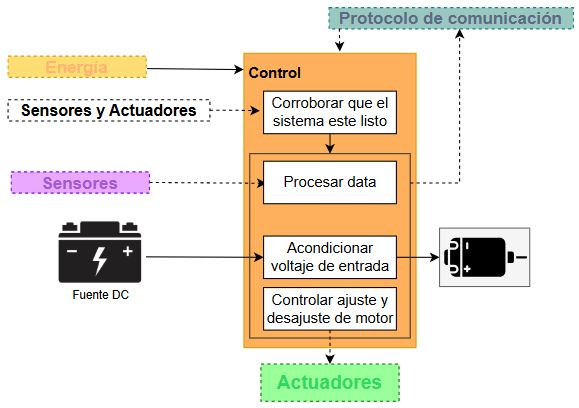
\includegraphics[width=\linewidth]{CHPTRS/CH03_DICON/Fig/CH03_FIG01_EstructuraDeFunciones/04_EstructuraDeFunciones-Control.JPG}
            \end{subfigure}
        \end{tabularx}
        \caption{Dominio de control}
        \label{fig:control}
    \end{figure}
\subsection{Dominio de Sensores}

    \noindent
    En este dominio, se busca principalmente censar los valores físicos de las variables que se usarán para la estimación de parámetros de motor, los cuales son: corriente $i(t)$, velocidad angular $\omega(t)$ y voltaje $u(t)$. Adicionalmente, se cuenta con una función que ayudará al sistema a validar que un motor ha sido correctamente fijado antes de iniciar con el proceso de caracterización. Como ya se mencionó, en la literatura, será necesario el uso de estas variables para poder estimar los parámetros usando los algoritmos necesarios para reconstruir un modelo lo más preciso posible del motor. Al contar con sensores precisos, favorecerá la exactitud del modelo. Si bien este punto puede ser bastante debatible, el uso de un buen sensor se debe acoplar al requerimiento de costos de la solución, ya que usualmente el precio de estos es proporcional a la resolución que tenga para la toma de datos. En la Figura \ref{fig:sensores}, se muestra el dominio descrito.
    \begin{figure}[H]
        \centering
        \begin{tabularx}{\linewidth}{>{\centering\arraybackslash}X}
            % Fila 1: imagen
            \begin{subfigure}[t]{0.8\linewidth}
                \centering
                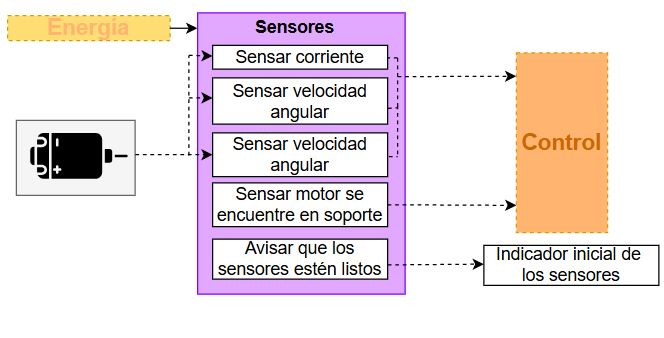
\includegraphics[width=\linewidth]{CHPTRS/CH03_DICON/Fig/CH03_FIG01_EstructuraDeFunciones/05_EstructuraDeFunciones-Sensores.JPG}
            \end{subfigure}
        \end{tabularx}
        \caption{Dominio de sensores}
        \label{fig:sensores}
    \end{figure}
\subsection{Dominio de Actuadores}

    \noindent
    Este dominio se encargará de ejecutar las acciones en el \ac{HW}. Este dominio también será energizado por la línea de potencia de $220\text{VAC }60\text{Hz}$ y las funciones que cumple este dominio son: 
    \begin{itemize}
        \item Notificar al usuario y al dominio de control que este dominio está operativo, mediante una señal digital para el controlador y un componente óptico (como un LED) o sonoro (como un \textit{buzzer}) para el usuario.
        \item Activar una parada de emergencia en caso de falla por sobre corriente para la protección del usuario.
        \item Sujetar correctamente el motor a analizar, como se mencionó en la sec. \ref{sec:CH04_Dominio_Cntrl}, se busca que durante la toma de datos para la identificación de sus parámetros el motor quede fijo ya sea por algún mecanismo que utilice al actuador o en su defecto manualmente. Este acople del motor se busca que sea lo más estándar posible para motores que se encuentren en el rango de voltaje definido $3-12 V$ como se mencionó en la Tabla \ref{tab:CH04_LISTA} lista de requerimientos .
    \end{itemize}
    En la Figura \ref{fig:ACTUADORES} se muestra el dominio de actuadores del sistema.
    \begin{figure}[H]
        \centering
        \begin{tabularx}{\linewidth}{>{\centering\arraybackslash}X}
            % Fila 1: imagen
            \begin{subfigure}[t]{0.8\linewidth}
                \centering
                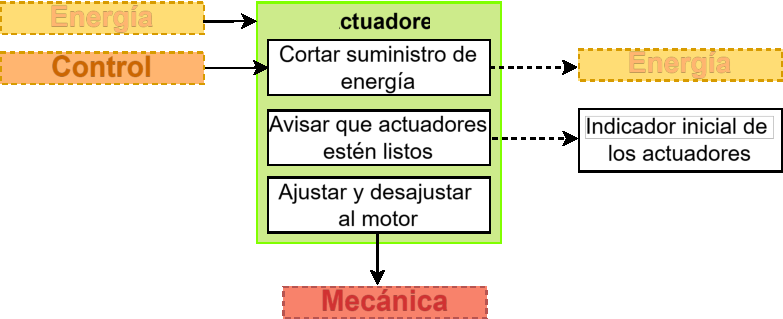
\includegraphics[width=\linewidth]{CHPTRS/CH03_DICON/Fig/CH03_FIG01_EstructuraDeFunciones/06_EstructuraDeFunciones-Actuadores.pdf}
            \end{subfigure}
        \end{tabularx}
        \caption{Dominio de actuadores}
        \label{fig:ACTUADORES}
    \end{figure}
\subsection{Dominio Mecánico}

    \noindent
    El dominio mecánico se encarga del diseño de las estructuras que soportarán a los componentes del sistema como al motor que será analizado. Se deberá diseñar adecuadamente el soporte del motor, minimizando las vibraciones generadas al momento de ser energizado, y así garantizar una toma de datos ininterrumpida y estable. Además, el diseño debe considerar soluciones eficientes de disipación de calor y ventilación, ya que varios componentes serán energizados simultáneamente, lo que puede generar un elevado consumo de corriente. Este dominio estará conectado al actuador que logre la fijación correcta del motor por analizar. El soporte del motor deberá ser adaptable, ya que en el mercado existe una amplia variedad de tamaños de motores  con un voltaje nominal de hasta \SI{12}{V}. Se espera que el sistema de fijación sea versátil y capaz de acomodar motores \ac{DC} de diferentes diámetros, garantizando la estabilidad mecánica en el análisis de sus parámetros. Como se muestra en la Figura \ref{fig:mecanica} el dominio mecánico puede ser extendido a demás dominios que necesiten de alguna estructura para el correcto ensamble de los componentes.
    \begin{figure}[H]
        \centering
        \begin{tabularx}{\linewidth}{>{\centering\arraybackslash}X}
            % Fila 1: imagen
            \begin{subfigure}[t]{0.9\linewidth}
                \centering
                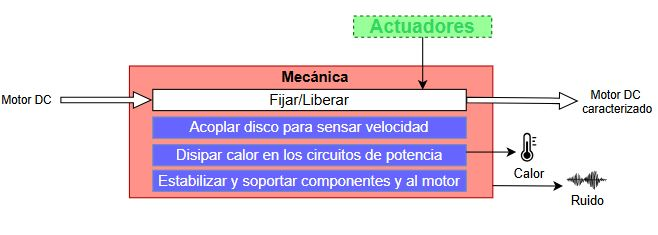
\includegraphics[width=\linewidth]{CHPTRS/CH03_DICON/Fig/CH03_FIG01_EstructuraDeFunciones/07_EstructuraDeFunciones-Mecanica.JPG}
            \end{subfigure}
        \end{tabularx}
        \caption{Dominio mecánico}
        \label{fig:mecanica}
    \end{figure}
\subsection{Dominio de Energía}

    \noindent
   En este dominio, la energía eléctrica de $220\text{VAC }60\text{Hz}$, correspondiente al estándar en Perú, es la fuente de alimentación de todo el sistema y se acondiciona para cumplir con los requerimientos de los componentes electrónicos, tales como actuadores, sensores y el controlador de la parte de \ac{HW} del sistema. El proceso inicia con la activación del sistema a través de un \textit{switch} o pulsador, que permite la entrada de la línea de potencia al sistema. A partir de este punto, durante la operación, el suministro de energía puede interrumpirse mediante una señal de parada de emergencia si se presenta algún problema que pueda dañar el motor, algún componente, o, más importante, comprometer la seguridad del usuario. Esta acción es gestionada por un dispositivo dentro del dominio de actuadores. La energía rectificada se utilizará para alimentar los componentes de los dominios de actuadores, sensores y control, como se ilustra en la Figura \ref{fig:dominio_Energia}.
    \begin{figure}[H]
        \centering
        \begin{tabularx}{\linewidth}{>{\centering\arraybackslash}X}
            % Fila 1: imagen
            \begin{subfigure}[t]{0.9\linewidth}
                \centering
                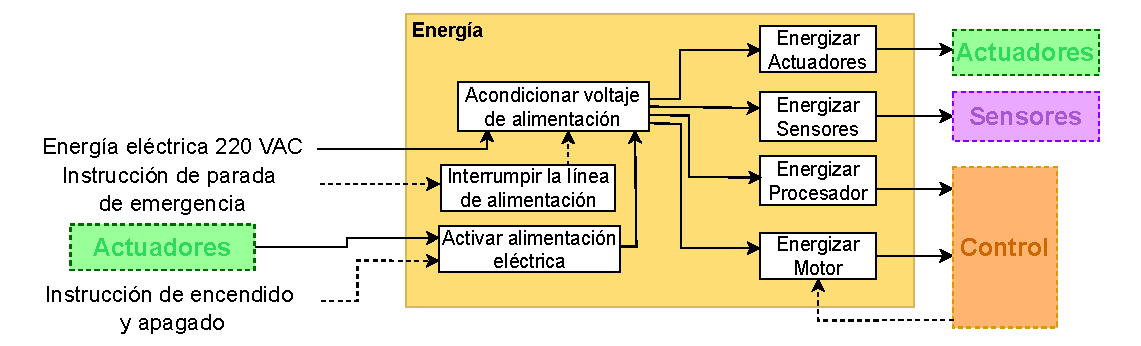
\includegraphics[width=\linewidth]{CHPTRS/CH03_DICON/Fig/CH03_FIG01_EstructuraDeFunciones/08_EstructuraDeFunciones-Energia.pdf}
            \end{subfigure}
        \end{tabularx}
        \caption{Dominio de energía}
        \label{fig:dominio_Energia}
    \end{figure}
